Da es sich bei dem Signal um eine statistische Größe handelt, wird eine gaußförmig Funktion benutzt, um das Signal zu beschreiben.
%Der Mittelwert der Signalfunktion stellt einen freien Parameter dar und entspricht im Optimalfall der $\pi^{0}$-Masse.
%Als zwei weitere freie Parameter werden die Amplitude der Signalfunktion, sowie die Standardabweichung vom Mittelwert benutzt.
\newline
Die \textit{Tail} Komponente wird durch eine exponentielle Funktion und einer gaußförmigen Funktion beschrieben.
Sie dient der Abschätzung des Anteils des Signals, dem Konversionselektronen oder Konversionspositronen zu Grunde liegen.
\newline
Für die Abschätzung des korrelierten Untergrund wird eine lineare Funktion angenommen.
\newline
Die drei Funktionen werden zusammen an die Verteilung angepasst.
\begin{figure}[tp]
\centering
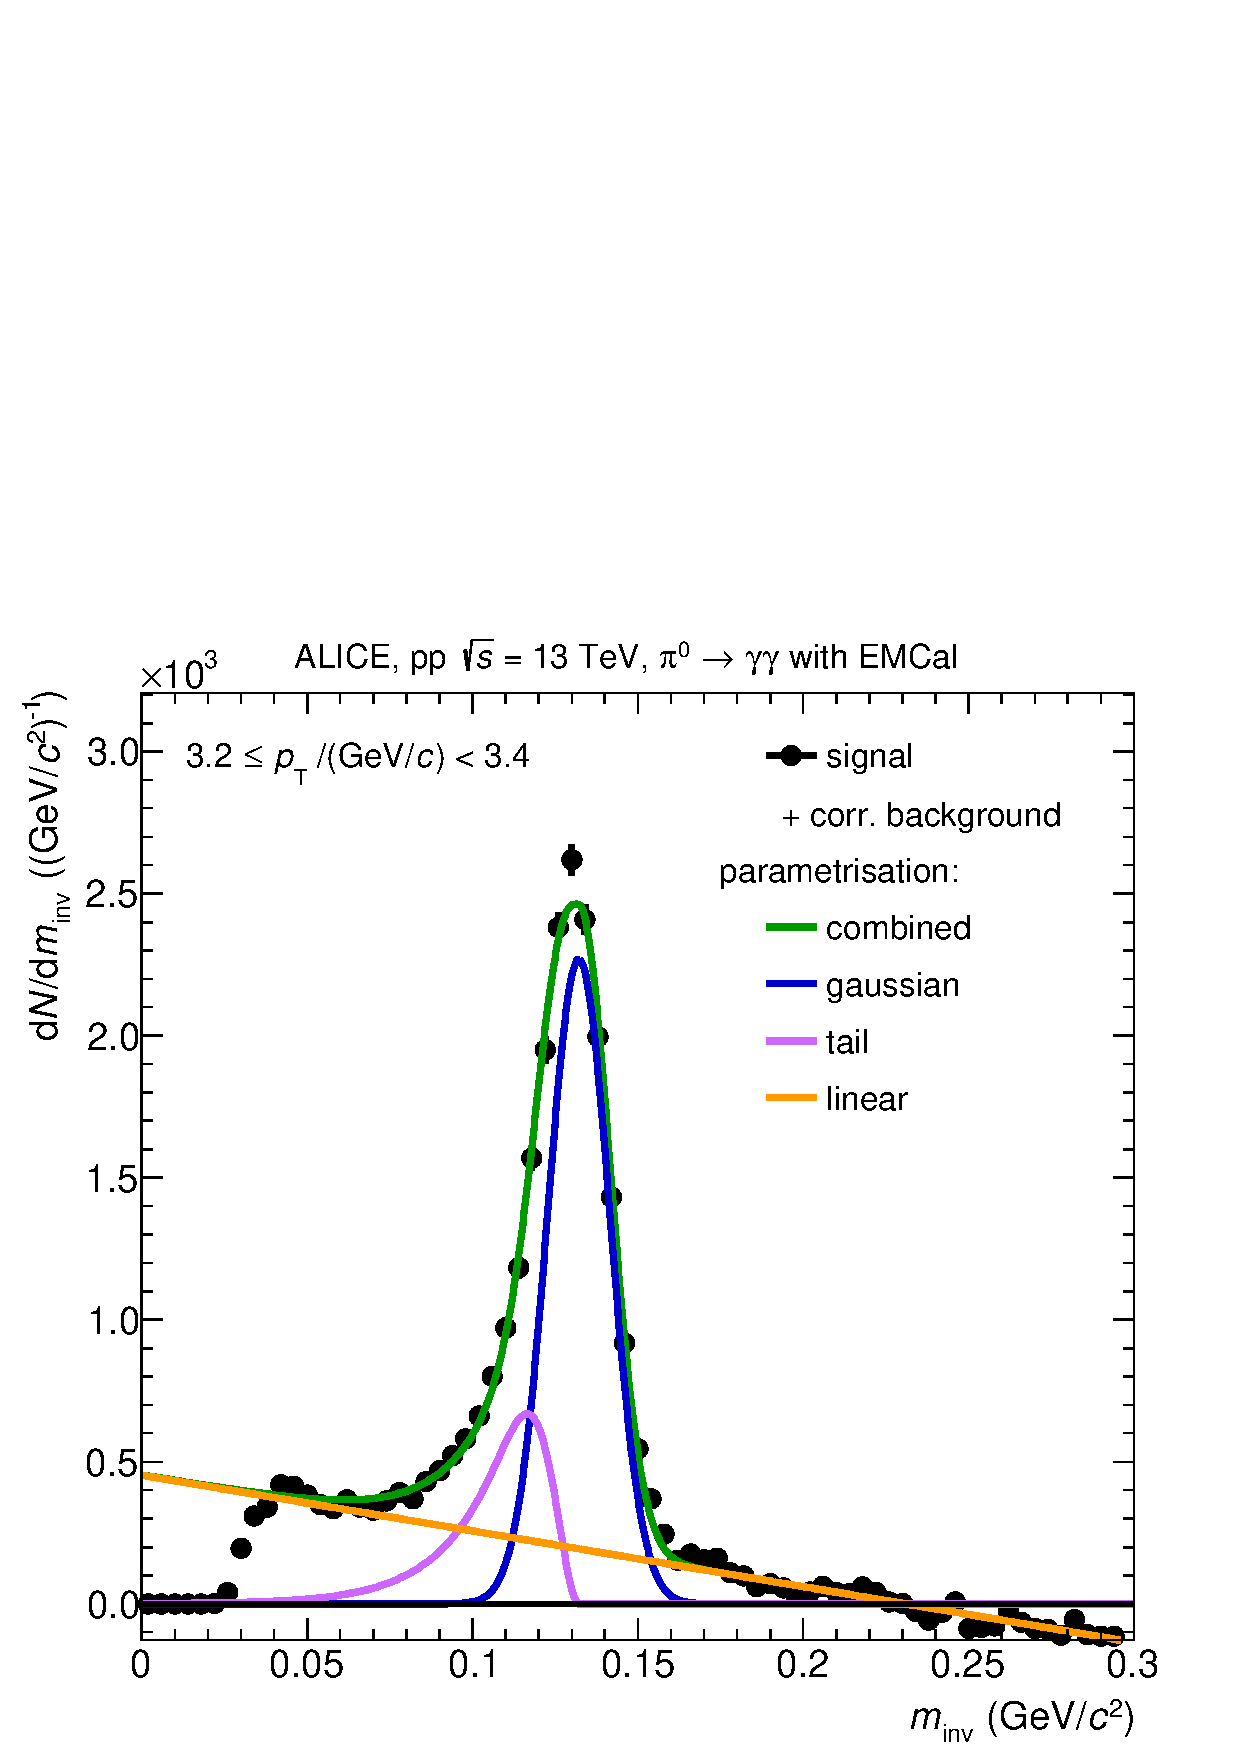
\includegraphics[width=.75\linewidth]{StandardParam.pdf}
\caption{Signal mit korreliertem Untergrund sowie den Funktionen zur Beschreibung des Signals mit korreliertem Untergrund.}
\label{figStandardParam}
\end{figure}
\newline
Abbildung \ref{figStandardParam} zeigt die Verteilung der invariante Masse bestehend aus Signal und korreliertem Untergrund, sowie das Ergebnis der an die Daten angepassten Funktion.
Die grüne Funktion entspricht der Summe der drei einzelnen Komponenten, wobei die Gauß-Funktion in blau, die \textit{Tail}-Funktion in pink und die lineare Funktion in orange, dargestellt werden.
Dabei wird deutlich, dass durch die Abschätzung des korrelierten Untergrunds über die lineare Funktion bei einer invarianten Masse von etwa $0\,06\text{ GeV}/c^{2}$, kein beziehungsweise kaum Signal mit dieser Methode erwartet wird.
Zu noch kleineren Massen hin sorgen die Anforderungen an den Öffnungswinkel dafür, dass die Datenpunkte rapide abnehmen, bis keine mehr da sind.
Dieses Verhalten wird nicht von der Abschätzung des korrelierten Untergrunds berücksichtigt.
\newline
Um die Anzahl der produzierten $\pi^{0}$ mit der Standardmethode zu bestimmen, wird zunächst die lineare Parametrisierung von den Daten abgezogen.
Anschließend werden die übrigen Daten, also das Signal, über einen festen Bereich um den Erwartungswert der Gauß-Funktion integriert.
Für eine detaillierte Beschreibung der Standardmethode sei an dieser Stelle auf \cite{thesis:Adrian} verwiesen.
\newline
Im folgenden Abschnitt wird die Abschätzung des korrelierten Untergrunds mit Hilfe von Templates beschrieben.